\documentclass{beamer}

\usetheme{Warsaw}
\usecolortheme{dove}
\usefonttheme{serif}
\usepackage{tikz}
\useinnertheme{rectangles}
\useoutertheme{miniframes}
\setbeamercolor*{mini frame}{fg=black,bg=white}
\setbeamercolor{section in head/foot}{fg=black, bg=white}


% Declare lengths

\newlength{\leafnodewidth} 
\newlength{\leafnodeheightone} 
\newlength{\leafnodeheighttwo}

\newlength{\leafnodetextstart}
\newlength{\leafnodetextend}

\newlength{\internalnoderadius}

\newlength{\leveldistance}

% Set length values

\setlength{\leafnodewidth}{6mm}
\setlength{\leafnodeheightone}{3mm}
\setlength{\leafnodeheighttwo}{9mm} 

\setlength{\leafnodetextstart}{11mm}
\setlength{\leafnodetextend}{15mm}

\setlength{\internalnoderadius}{3.5mm}

\setlength{\leveldistance}{14mm}

% Declare colors
\definecolor{leafcolorone}{RGB}{255,0,0} % red
\definecolor{leafcolortwo}{RGB}{0,0,255} % blue
\definecolor{internalnodecolor}{RGB}{0,255,0} % green
\definecolor{highlightededgecolor}{RGB}{139,1,102} %dark magenta

\addtobeamertemplate{navigation symbols}{}{%
	\usebeamerfont{footline}%
	\usebeamercolor[fg]{footline}%
	\hspace{1em}%
	\insertframenumber/\inserttotalframenumber
}

% Define the \leafnode command
\newcommand{\leafnode}[6]{
	\begin{tikzpicture}
		\filldraw[color=#1!90, fill=#1!3, thick, font=\tiny] (0,0) rectangle (\leafnodewidth, -\leafnodeheightone) node[midway, text=#3] {#4};
		\filldraw[color=#2!90, fill=#2!3, thick, font=\small] (0,-\leafnodeheightone) rectangle (\leafnodewidth, -\leafnodeheighttwo) node[midway, text=#3] {#5};

        % the following portion is only for showing after demonstration
        
		%\filldraw[color=white!100, fill=white!100, thick, font=\scriptsize] (0,-\leafnodetextstart) rectangle (\leafnodewidth, -\leafnodetextend) node[midway, text=#3] {#6};
  
	\end{tikzpicture}
}


% Define the \leafnode command
\newcommand{\labelledleafnode}[6]{
	\begin{tikzpicture}
		\filldraw[color=#1!90, fill=#1!3, thick, font=\tiny] (0,0) rectangle (\leafnodewidth, -\leafnodeheightone) node[midway, text=#3] {#4};
		\filldraw[color=#2!90, fill=#2!3, thick, font=\small] (0,-\leafnodeheightone) rectangle (\leafnodewidth, -\leafnodeheighttwo) node[midway, text=#3] {#5};
        
		\filldraw[color=violet!100, fill=white!100, thick, font=\scriptsize] (0,-\leafnodetextstart) rectangle (\leafnodewidth, -\leafnodetextend) node[midway, text=#3] {#6};
  
	\end{tikzpicture}
}

% Define the \internalnode command with a color argument
\newcommand{\internalnode}[3]{
	\begin{tikzpicture}
		\filldraw[color=#1!90, fill=#1!5, thick, font=\scriptsize] (0,0) circle (\internalnoderadius) node[midway, text=#2] {#3};
	\end{tikzpicture}
}


% Minimum Indicator
\newcommand{\mindicator}[0]{

\vspace{0.5mm}

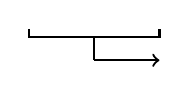
\begin{tikzpicture}

\draw[black, thick] (0,0.1) -- (0,0) -- (1.66,0) -- (1.66,0.1);
\draw[black, thick] (0.83,0) -- (0.83,-0.3);
\draw[black, thick, ->] (0.83,-0.3) -- (1.66,-0.3);
% Adding a dummy line for better positioning of the text
\draw[white] (0,-0.4) -- (1.66,-0.4);

\end{tikzpicture}
\footnotesize{Minimum-weighted two nodes. Now these will be combined\ldots}
% \begin{tikzpicture}
% \node[draw=white, fill=white, rectangle, font=\footnotesize] at (0,0) {Minimum};
% \end{tikzpicture}

}


\begin{document}




\tikzstyle{level 1} = [sibling distance=38mm]
\tikzstyle{level 2} = [sibling distance=30mm]
\tikzstyle{level 3} = [sibling distance=19mm]
\tikzstyle{visible_edge} = [->, draw, leafcolortwo, thick]
\tikzstyle{edge from parent} = [draw, teal, thick]
\tikzstyle{emph} = [edge from parent/.style={->,highlightededgecolor,draw,ultra thick}]
\tikzstyle{norm} = [edge from parent/.style={draw, teal, thin}]
\tikzstyle{noedge} = [edge from parent/.style={draw, white, thin}]

\tikzstyle{every node} = [inner sep=0]


% Construction of Huffman Tree

\section{Construction of Huffman Tree}


% Frame 1 - Only leaf nodes
\begin{frame}[c]{Construction of Huffman Tree}

\leafnode{leafcolorone}{leafcolortwo}{black}{0.15}{D}{010}
\leafnode{leafcolorone}{leafcolortwo}{black}{0.16}{E}{011}
\leafnode{leafcolorone}{leafcolortwo}{black}{0.17}{A}{000}
\leafnode{leafcolorone}{leafcolortwo}{black}{0.17}{C}{001}
\leafnode{leafcolorone}{leafcolortwo}{black}{0.35}{B}{1}

\mindicator

\end{frame} 



% Frame 2 - One merge
\begin{frame}[c]{Construction of Huffman Tree}

\onslide <2>
\leafnode{leafcolorone}{leafcolortwo}{black}{0.17}{A}{000}
\leafnode{leafcolorone}{leafcolortwo}{black}{0.17}{C}{001}
\internalnode{internalnodecolor}{black}{0.31}
\leafnode{leafcolorone}{leafcolortwo}{black}{0.35}{B}{1}

\mindicator

\onslide <1->
 
	\begin{figure}
		
		\begin{tikzpicture}[
			level distance=\leveldistance
			]
			
			\node {\internalnode{white}{white}{1.00}}
			child[noedge]{
				node {\internalnode{white}{white}{0.65}}
				child[noedge]{
					node {\internalnode{white}{white}{0.34}}
					child[noedge]{
						node {\leafnode{white}{white}{white}{0.17}{A}{000}}
					}
					child[noedge]{
						node {\leafnode{white}{white}{white}{0.17}{C}{001}}
					}
				}
				child[noedge]{
					node {\internalnode{internalnodecolor}{black}{0.31}}
					child[norm]{
						node {\leafnode{leafcolorone}{leafcolortwo}{black}{0.15}{D}{010}}
					}
					child[norm]{
						node {\leafnode{leafcolorone}{leafcolortwo}{black}{0.16}{E}{011}}
					}
				}
			}
			child[noedge]{
				node {\leafnode{white}{white}{white}{0.35}{B}{1}}
			};
			
		\end{tikzpicture}
		
	\end{figure}
	
	
\end{frame}




% Frame 3 - Two merges
\begin{frame}[c]{Construction of Huffman Tree}

\onslide <2>
\internalnode{internalnodecolor}{black}{0.31}
\internalnode{internalnodecolor}{black}{0.34}
\leafnode{leafcolorone}{leafcolortwo}{black}{0.35}{B}{1}

\mindicator

\onslide <1->
	\begin{figure}
		
		\begin{tikzpicture}[
			level distance=\leveldistance
			]
			
			\node {\internalnode{white}{white}{1.00}}
			child[noedge]{
				node {\internalnode{white}{white}{0.65}}
				child[noedge]{
					node {\internalnode{internalnodecolor}{black}{0.34}}
					child[norm]{
						node {\leafnode{leafcolorone}{leafcolortwo}{black}{0.17}{A}{000}}
					}
					child[norm]{
						node {\leafnode{leafcolorone}{leafcolortwo}{black}{0.17}{C}{001}}
					}
				}
				child[noedge]{
					node {\internalnode{internalnodecolor}{black}{0.31}}
					child[norm]{
						node {\leafnode{leafcolorone}{leafcolortwo}{black}{0.15}{D}{010}}
					}
					child[norm]{
						node {\leafnode{leafcolorone}{leafcolortwo}{black}{0.16}{E}{011}}
					}
				}
			}
			child[noedge]{
				node {\leafnode{white}{white}{white}{0.35}{B}{1}}
			};
			
		\end{tikzpicture}
		
	\end{figure}
	
	
\end{frame}




% Frame 4 - Three merges
\begin{frame}[c]{Construction of Huffman Tree}

\onslide <2>
\leafnode{leafcolorone}{leafcolortwo}{black}{0.35}{B}{1}
\internalnode{internalnodecolor}{black}{0.65}

\mindicator

\onslide <1->
	\begin{figure}
		
		\begin{tikzpicture}[
			level distance=\leveldistance
			]
			
			\node {\internalnode{white}{white}{1.00}}
			child[noedge]{
				node {\internalnode{internalnodecolor}{black}{0.65}}
				child[norm]{
					node {\internalnode{internalnodecolor}{black}{0.34}}
					child[norm]{
						node {\leafnode{leafcolorone}{leafcolortwo}{black}{0.17}{A}{000}}
					}
					child[norm]{
						node {\leafnode{leafcolorone}{leafcolortwo}{black}{0.17}{C}{001}}
					}
				}
				child[norm]{
					node {\internalnode{internalnodecolor}{black}{0.31}}
					child[norm]{
						node {\leafnode{leafcolorone}{leafcolortwo}{black}{0.15}{D}{010}}
					}
					child[norm]{
						node {\leafnode{leafcolorone}{leafcolortwo}{black}{0.16}{E}{011}}
					}
				}
			}
			child[noedge]{
				node {\leafnode{white}{white}{white}{0.35}{B}{1}}
			};
			
		\end{tikzpicture}
		
	\end{figure}
	
	
\end{frame}






% Final Frame
\begin{frame}[c]{Construction of Huffman Tree}
	
	\begin{figure}
		
		\begin{tikzpicture}[
			level distance=\leveldistance
			]
			
			\node {\internalnode{internalnodecolor}{black}{1.00}}
			child[norm]{
				node {\internalnode{internalnodecolor}{black}{0.65}}
				child[norm]{
					node {\internalnode{internalnodecolor}{black}{0.34}}
					child[norm]{
						node {\leafnode{leafcolorone}{leafcolortwo}{black}{0.17}{A}{000}}
					}
					child[norm]{
						node {\leafnode{leafcolorone}{leafcolortwo}{black}{0.17}{C}{001}}
					}
				}
				child[norm]{
					node {\internalnode{internalnodecolor}{black}{0.31}}
					child[norm]{
						node {\leafnode{leafcolorone}{leafcolortwo}{black}{0.15}{D}{010}}
					}
					child[norm]{
						node {\leafnode{leafcolorone}{leafcolortwo}{black}{0.16}{E}{011}}
					}
				}
			}
			child[norm]{
				node {\leafnode{leafcolorone}{leafcolortwo}{black}{0.35}{B}{1}}
			};
			
		\end{tikzpicture}
		
	\end{figure}
	
	
\end{frame}



\section{Interpreting Binary Codes}



\begin{frame}[c]{Interpreting Binary Codes}

\begin{example}
    Let's say we want to find the binary encoding of the letter 'D'
\end{example} 
    
	\begin{figure}
		
		\begin{tikzpicture}[
			level distance=\leveldistance
			]

            \onslide <2>
            
			\node {\internalnode{internalnodecolor}{black}{1.00}}
			child[norm]{
				node {\internalnode{internalnodecolor}{black}{0.65}}
				child[norm]{
					node {\internalnode{internalnodecolor}{black}{0.34}}
					child[norm]{
						node {\leafnode{leafcolorone}{leafcolortwo}{black}{0.17}{A}{000}}
					}
					child[norm]{
						node {\leafnode{leafcolorone}{leafcolortwo}{black}{0.17}{C}{001}}
					}
				}
				child[norm]{
					node {\internalnode{internalnodecolor}{black}{0.31}}
					child[norm]{
						node {\leafnode{leafcolorone}{leafcolortwo}{black}{0.15}{D}{010}}
					}
					child[norm]{
						node {\leafnode{leafcolorone}{leafcolortwo}{black}{0.16}{E}{011}}
					}
				}
			}
			child[norm]{
				node {\leafnode{leafcolorone}{leafcolortwo}{black}{0.35}{B}{1}}
			};



            \onslide <3>
            
			\node {\internalnode{internalnodecolor}{black}{1.00}}
			child[emph]{
				node {\internalnode{internalnodecolor}{black}{0.65}}
				child[norm]{
					node {\internalnode{internalnodecolor}{black}{0.34}}
					child[norm]{
						node {\leafnode{leafcolorone}{leafcolortwo}{black}{0.17}{A}{000}}
					}
					child[norm]{
						node {\leafnode{leafcolorone}{leafcolortwo}{black}{0.17}{C}{001}}
					}
				}
				child[norm]{
					node {\internalnode{internalnodecolor}{black}{0.31}}
					child[norm]{
						node {\leafnode{leafcolorone}{leafcolortwo}{black}{0.15}{D}{010}}
					}
					child[norm]{
						node {\leafnode{leafcolorone}{leafcolortwo}{black}{0.16}{E}{011}}
					}
				}
			}
			child[norm]{
				node {\leafnode{leafcolorone}{leafcolortwo}{black}{0.35}{B}{1}}
			};


            \onslide <4>
            
			\node {\internalnode{internalnodecolor}{black}{1.00}}
			child[emph]{
				node {\internalnode{internalnodecolor}{black}{0.65}}
				child[norm]{
					node {\internalnode{internalnodecolor}{black}{0.34}}
					child[norm]{
						node {\leafnode{leafcolorone}{leafcolortwo}{black}{0.17}{A}{000}}
					}
					child[norm]{
						node {\leafnode{leafcolorone}{leafcolortwo}{black}{0.17}{C}{001}}
					}
				}
				child[emph]{
					node {\internalnode{internalnodecolor}{black}{0.31}}
					child[norm]{
						node {\leafnode{leafcolorone}{leafcolortwo}{black}{0.15}{D}{010}}
					}
					child[norm]{
						node {\leafnode{leafcolorone}{leafcolortwo}{black}{0.16}{E}{011}}
					}
				}
			}
			child[norm]{
				node {\leafnode{leafcolorone}{leafcolortwo}{black}{0.35}{B}{1}}
			};



            \onslide <5>
            
			\node {\internalnode{internalnodecolor}{black}{1.00}}
			child[emph]{
				node {\internalnode{internalnodecolor}{black}{0.65}}
				child[norm]{
					node {\internalnode{internalnodecolor}{black}{0.34}}
					child[norm]{
						node {\leafnode{leafcolorone}{leafcolortwo}{black}{0.17}{A}{000}}
					}
					child[norm]{
						node {\leafnode{leafcolorone}{leafcolortwo}{black}{0.17}{C}{001}}
					}
				}
				child[emph]{
					node {\internalnode{internalnodecolor}{black}{0.31}}
					child[emph]{
						node {\leafnode{leafcolorone}{leafcolortwo}{black}{0.15}{D}{010}}
					}
					child[norm]{
						node {\leafnode{leafcolorone}{leafcolortwo}{black}{0.16}{E}{011}}
					}
				}
			}
			child[norm]{
				node {\leafnode{leafcolorone}{leafcolortwo}{black}{0.35}{B}{1}}
			};
            


   
			
		\end{tikzpicture}
		
	\end{figure}
	
	
\end{frame}


\begin{frame}[c]{Interpreting Binary Codes}

\begin{example}
    So, the binary encoding of 'D' = 010
\end{example} 
    
	\begin{figure}
		
		\begin{tikzpicture}[
			level distance=\leveldistance
			]

            \node {\internalnode{internalnodecolor}{black}{1.00}}
			child[emph]{
				node {\internalnode{internalnodecolor}{black}{0.65}}
				child[norm]{
					node {\internalnode{internalnodecolor}{black}{0.34}}
					child[norm]{
						node {\leafnode{leafcolorone}{leafcolortwo}{black}{0.17}{A}{000}}
					}
					child[norm]{
						node {\leafnode{leafcolorone}{leafcolortwo}{black}{0.17}{C}{001}}
					}
				}
				child[emph]{
					node {\internalnode{internalnodecolor}{black}{0.31}}
					child[emph]{
						node {\leafnode{leafcolorone}{leafcolortwo}{black}{0.15}{D}{010}}
					}
					child[norm]{
						node {\leafnode{leafcolorone}{leafcolortwo}{black}{0.16}{E}{011}}
					}
				}
			}
			child[norm]{
				node {\leafnode{leafcolorone}{leafcolortwo}{black}{0.35}{B}{1}}
			};
  
        \end{tikzpicture}

    \end{figure}

\end{frame}


\setbeamercovered{transparent}
\begin{frame}{Interpreting Binary Codes}
\begin{block}{}
    Similarly, we determine all the codes\ldots
\end{block} 
    \centering
    \begin{table}
        % \onslide<1->\caption{\textbf{Complexity Comparison}}
        \begin{tabular}{c|c}
            \hline
            \hline
            \onslide<1-> \textbf{Letter} & \textbf{Binary Code} \\
            \hline
            \hline
            \onslide<2-> A & 000  \\
            %				\hline
            \onslide<3->
            B & 1  \\
            %				\hline
            \onslide<4->
            C & 001 \\
            %				\hline
            \onslide<5->
            D & 010 \\
            %				\hline
            \onslide<6->
            E & 011 
            %				\hline
        \end{tabular}
    \end{table}
\end{frame}



% Final Frame containing all leaf label binary codes
\begin{frame}[c]{Interpreting Binary Codes}

\begin{block}{}
    Similarly, we determine all the codes\ldots
\end{block} 

	\begin{figure}
		
		\begin{tikzpicture}[
			level distance=\leveldistance
			]
			
			\node {\internalnode{internalnodecolor}{black}{1.00}}
			child[norm]{
				node {\internalnode{internalnodecolor}{black}{0.65}}
				child[norm]{
					node {\internalnode{internalnodecolor}{black}{0.34}}
					child[norm]{
						node {\labelledleafnode{leafcolorone}{leafcolortwo}{black}{0.17}{A}{000}}
					}
					child[norm]{
						node {\labelledleafnode{leafcolorone}{leafcolortwo}{black}{0.17}{C}{001}}
					}
				}
				child[norm]{
					node {\internalnode{internalnodecolor}{black}{0.31}}
					child[norm]{
						node {\labelledleafnode{leafcolorone}{leafcolortwo}{black}{0.15}{D}{010}}
					}
					child[norm]{
						node {\labelledleafnode{leafcolorone}{leafcolortwo}{black}{0.16}{E}{011}}
					}
				}
			}
			child[norm]{
				node {\labelledleafnode{leafcolorone}{leafcolortwo}{black}{0.35}{B}{1}}
			};
			
		\end{tikzpicture}
		
	\end{figure}
	
	
\end{frame}



\end{document}